\subsubsection{Prospetto Orario}
Di seguito è riportata la suddivisione oraria dei ruoli durante l'intera durata del periodo rendicontato del progetto.


\begin{table}[H]	
	\begin{center}
	    \begin{tabular}{cccccccc}
			\rowcolor{greySWEight}
			\textcolor{white}{\textbf{Nome}} & \textcolor{white}{\textbf{Re}} & \textcolor{white}{\textbf{Am}} & \textcolor{white}{\textbf{An}} & \textcolor{white}{\textbf{Pj}} & \textcolor{white}{\textbf{Pr}} & \textcolor{white}{\textbf{Ve}} & \textcolor{white}{\textbf{Totale}}
			\\			

%			Bacco Alberto & 5 & 0 & 17 & 27 & 10 & 44 & 103 \\
%			Caccaro Sebastiano & 5 & 5 & 0 & 12 & 32 & 49 & 103 \\
%			Ciagola Damien & 5 & 5 & 0 & 39 & 12 & 42 & 103 \\
%			Corti Francesco & 5 & 10 & 5 & 15 & 22 & 46 & 103 \\
%			Isachi Gheorghe & 5 & 0 & 0 & 36 & 20 & 42 & 103 \\
%			Legrottagle Gionata & 0 & 0 & 0 & 49 & 20 & 34 & 103 \\
%			Magarotto Francesco & 5 & 5 & 0 & 56 & 12 & 25 & 103 \\
%			Muraro Enrico & 5 & 5 & 0 & 24 & 32 & 37 & 103 \\
			Bacco Alberto & 5 & 5 & 17 & 15 & 17 & 44 & 103 \\
			Caccaro Sebastiano & 0 & 5 & 0 & 31 & 18 & 49 & 103 \\
			Ciagola Damien & 5 & 0 & 0 & 32 & 24 & 42 & 103 \\
			Corti Francesco & 5 & 10 & 5 & 28 & 17 & 38 & 103 \\
			Isachi Gheorghe & 5 & 0 & 0 & 28 & 20 & 50 & 103 \\
			Legrottagle Gionata & 5 & 0 & 0 & 44 & 20 & 34 & 103 \\
			Magarotto Francesco & 5 & 5 & 0 & 41 & 27 & 25 & 103 \\
			Muraro Enrico & 5 & 5 & 0 & 39 & 17 & 37 & 103 \\
			\end{tabular}
	    \caption{Tabella della suddivisione oraria dei membri del gruppo nel periodo rendicontato del progetto} \label{tab:tabellaPersoneTotale} 
	\end{center}
\end{table}

La tabella della suddivisione oraria è rappresentata nel seguente grafico.
\begin{figure}[H]
	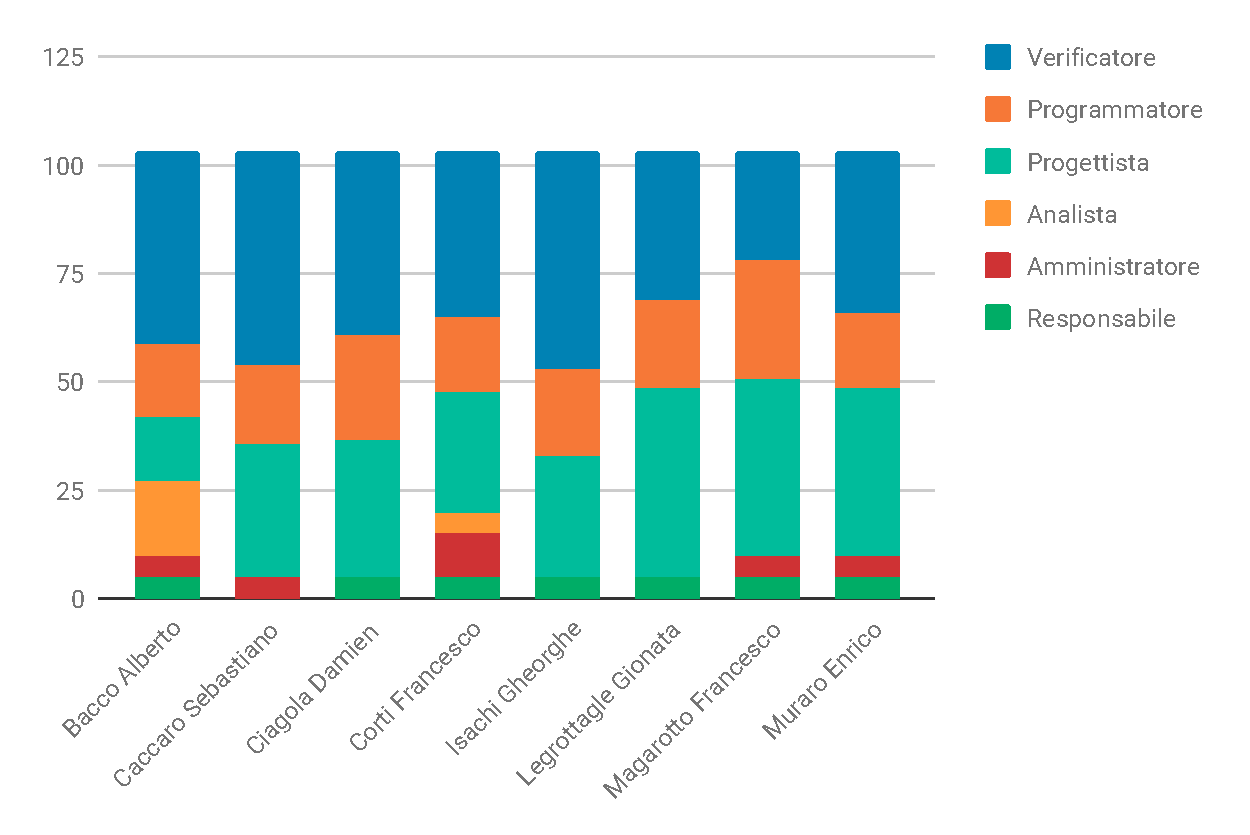
\includegraphics[width=1\linewidth]{Preventivo/grafici/TR1_2.pdf}
	\caption{Grafico della suddivisione oraria dei membri del gruppo nel periodo rendicontato del progetto}
\end{figure}

\subsubsection{Prospetto Economico}
Nella seguente tabella sono riportate le ore e i costi preventivati per ogni ruolo durante l'intera durata del periodo rendicontato del progetto.


\begin{table}[H]	
	\begin{center}
	    \begin{tabular}{C{4cm}C{1cm}C{3,5cm}}
			\rowcolor{greySWEight}
			\textcolor{white}{\textbf{Ruolo}} & \textcolor{white}{\textbf{Ore}} & \textcolor{white}{\textbf{Costo in €}}
			\\
			Responsabile & 35 & 1.050,00 \\
			Amministratore & 30 & 600,00 \\
			Analista & 22 & 550,00 \\
			Progettista & 258 & 5.676,00 \\
			Programmatore & 160 & 2.400,00 \\
			Verificatore & 319 & 4.785,00 \\
			\textbf{Totale} & \textbf{824} & \textbf{15.061,00} \\
		\end{tabular}
	    \caption{Tabella della suddivisione oraria dei ruoli nel periodo rendicontato del progetto} \label{tab:tabellaRuoliTotale} 
	\end{center}
\end{table}


Si può avere una più chiara rappresentazione della distribuzione oraria dei ruoli nel seguente grafico.

\begin{figure}[H]
	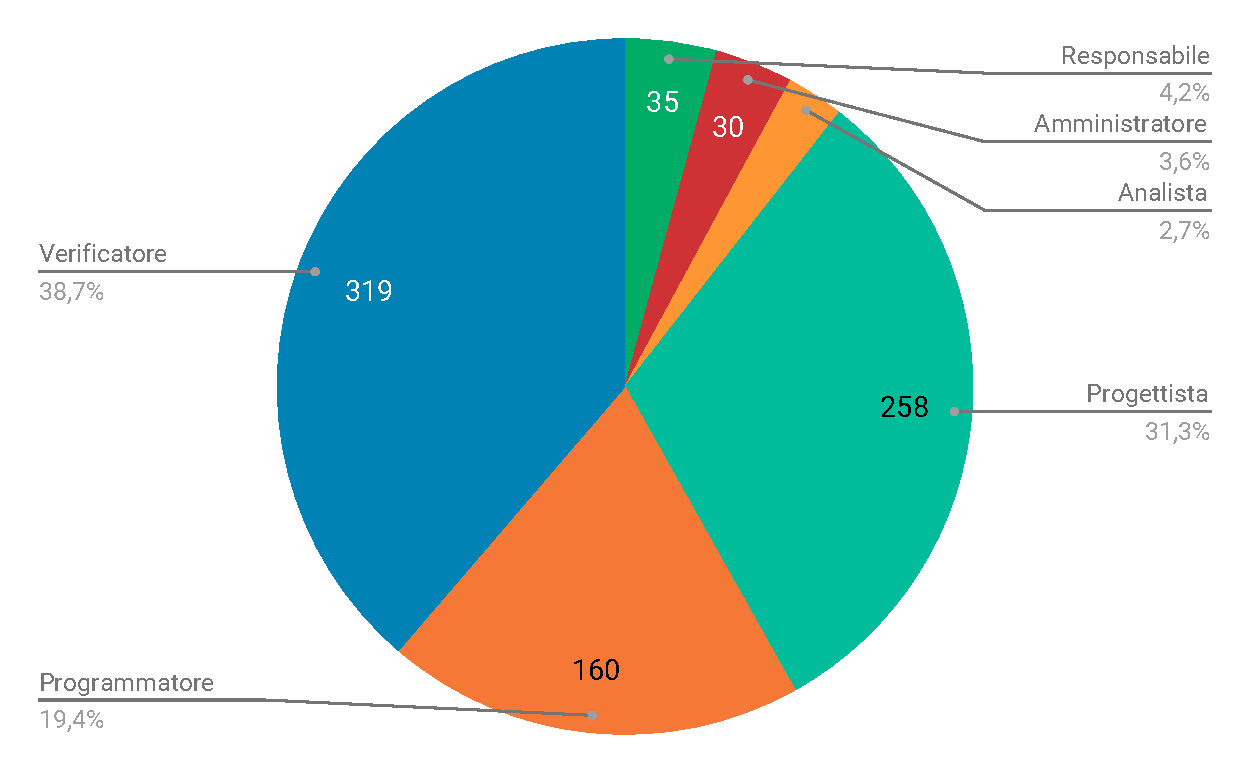
\includegraphics[width=1\linewidth]{Preventivo/grafici/TR2.pdf}
	\caption{Grafico della suddivisione oraria dei ruoli nel periodo rendicontato del progetto}
\end{figure}

